% Configuration du fichier final
%%%%%%%%%%%%%%%%%%%%%%%%%%%%%%%%%%%%%%%%%%%%%%%%%%%%%%%%%%%%%%%%%%%%%%%%%%%%%%%
%% Si vous voulez plus petit passez en 11pt voire encore plus petit en 10pt
\documentclass[a4paper,12pt,francais]{report}

%% Je suis francophone !
\usepackage[francais]{babel}
\usepackage[utf8x]{inputenc}
\usepackage[T1]{fontenc}
\selectlanguage{french}

%% J'ai besoin des paquet:
\usepackage{longtable,geometry,setspace}
\usepackage[francais]{layout}
\usepackage{listings}
\usepackage{lastpage}
\usepackage[francais]{varioref}
\usepackage{color}

%% J'aime bien pouvoir contrôler mes hauts de page !
\usepackage{fancyheadings}
\usepackage{fancyhdr}
\pagestyle{fancyplain}

%% Je veux pouvoir inclure des figures...
%% À commenter si vous voulez faire du DVI :
%

%% Quelques couleurs
\definecolor{titre}{gray}{0.4}
\definecolor{titre1}{gray}{0.5}
\definecolor{titre2}{gray}{0.6}
\definecolor{titre3}{gray}{0.7}
\definecolor{bleu}{rgb}{0.0,0.0,0.6}

%% Je veux créer des Hyperdocuments
%% À commenter si vous voulez faire du DVI :
%  [pdftex,colorlinks=true,linkcolor=blue,citecolor=blue,urlcolor=blue]
%\usepackage{hyperref}
\ifpdf
    \pdfoutput=1
    \pdfcompresslevel=9
    \usepackage[pdftex=true,
    hyperindex=true,
    colorlinks=true,
    pdfpagelabels,
    linkcolor=bleu,
    citecolor=red,
    urlcolor=bleu,
    anchorcolor=red,
    plainpages=false,
    bookmarks=true]{hyperref}
    % réglage des paramètres pour la création des pdf
    % à mettre dans l'entête du document
    \def\docpdf{
    \hypersetup{
      pdftitle={\@typerapport},
      pdfauthor={\@auteur},
      pdfsubject={\@titre},
    }}
    \usepackage[pdftex]{graphicx}
\else
    \usepackage[hypertex=true,
    hyperindex=true,
    colorlinks=false]{hyperref}
    \usepackage{graphicx}
\fi

%%%%%%%%%%%%%%%%%%%%%%%%%%%%%%%%%%%%%%%%%%%%%%%%%%%%%%%%%%%%%%%%%%%%%%%%%%%%%%%
%% Je peux définir mes propres « commandes »...

%% pour citer une figure :
\newcommand{\figref}[1]{(cf. Fig. \vref{#1})}

%% pour citer une équation :
\newcommand{\nref}[1]{(cf. \vref{#1})}

%% pour citer un livre:
\newcommand{\bibref}[1]{(cf. Bibliographie \cite{#1})}

%% pour mettre l'emphase sur un mot ou un groupe de mots :
\newcommand{\empha}[1]{\textit{\textbf{#1}}}

% Je regele les marges pour appliquer le standard EIGSI
\geometry{%
  a4paper,
  body={150mm,240mm},
  left=40mm,top=30mm,
  headheight=10mm,headsep=7mm,
  marginparsep=0mm,
  marginparwidth=0mm}
%% Je definie les numérotation   
\setcounter{secnumdepth}{3}

%% Voilà des hauts de page comme je les aime :
\fancyhf{} %initialise tous les champs dans head et foot
\chead{\small Representation du trafic aérien de Tahiti dans Google Earth}
\lhead{\thesection}
\rhead{\small DGAC}
\lfoot{\small Satge été 2010}
\rfoot{\small Page: \thepage\ sur \pageref{LastPage}}
\cfoot{M. \textsc{Kervizic} Emmanuel - \textsc{Promo}2011}
\renewcommand{\headrulewidth}{1pt}% met la largeur du trait à 1.5pt
\renewcommand{\footrulewidth}{1pt}

\fancypagestyle{plain}{%
\renewcommand{\headrulewidth}{1pt}% met la largeur du trait à 1.5pt
\renewcommand{\footrulewidth}{1pt}}

%% Voilà mes légendes de figures comme je les aime
\makeatletter
\def\figurename{{\protect\sc \protect\small\bfseries Fig.}}
\def\f@ffrench{\protect\figurename\space{\protect\small\bf \thefigure}\space}
\let\fnum@figure\f@ffrench%
\let\captionORI\caption
\def\caption#1{\captionORI{\rm\small #1}}
\makeatother

%% Je met en forme le code python importé
\lstset{ %
language=Python,                % choose the language of the code
basicstyle=\scriptsize,         % the size of the fonts that are used for the code
numbers=left,                   % where to put the line-numbers
numberstyle=\scriptsize,        % the size of the fonts that are used for the line-numbers
stepnumber=1,                   % the step between two line-numbers. If it's 1 each line 
                                % will be numbered
numbersep=5pt,                  % how far the line-numbers are from the code
backgroundcolor=\color{white},  % choose the background color. You must add \usepackage{color}
showspaces=false,               % show spaces adding particular underscores
showstringspaces=false,         % underline spaces within strings
showtabs=false,                 % show tabs within strings adding particular underscores
frame=single,	                % adds a frame around the code
tabsize=2,	                    % sets default tabsize to 2 spaces
captionpos=b,                   % sets the caption-position to bottom
breaklines=true,                % sets automatic line breaking
breakatwhitespace=false,        % sets if automatic breaks should only happen at whitespace
title=\lstname,                 % show the filename of files included with \lstinputlisting;
                                % also try caption instead of title
escapeinside={\%*}{*)},         % if you want to add a comment within your code
morekeywords={*,self},            % if you want to add more keywords to the set
keywordstyle=\bf \color {blue},
%identifierstyle=\underline,
commentstyle=\color[gray]{0.5},
stringstyle=\color{red},
extendedchars=\true,
inputencoding=utf8x
}


%%%%%%%%%%%%%%%%%%%%%%%%%%%%%%%%%%%%%%%%%%%%%%%%%%%%%%%%%%%%%%%%%%% 
% Définitions des variables et des macros pour les modifier pour la 
% page de titre. dans le texte, utiliser \wxxx pour ecrire xxx dans 
% le document, par exple : \wauteur ecrit l'auteur ...
% Période du stage
\def\@periode{Non renseigné~!}
\def\periode#1{\def\@periode{#1}}
\newcommand{\wperiode}{\@periode}
% Auteur du rapport
\def\@auteur{Non renseigné~!}
\def\auteur#1{\def\@auteur{#1}}
\newcommand{\wauteur}{\@auteur}
% Type de rapport (tfe, stage 2A, 3A, \ldots)
\def\@typerapport{Non renseigné~!}
\def\typerapport#1{\def\@typerapport{#1}}
\newcommand{\wtyperapport}{\@typerapport}
% Titre
\def\@titre{Non renseigné~!}
\def\titre#1{\def\@titre{#1}}
\newcommand{\wtitre}{\@titre}
% Tuteur entreprise
\def\@tuteurent{Non renseigné~!}
\def\tuteurent#1{\def\@tuteurent{#1}}
% Tuteur école
\def\@tuteurstage{Non renseigné~!}
\def\tuteurstage#1{\def\@tuteurstage{#1}}
% Logo entreprise (exple : logo_emac.png)
\def\@logoentrep{}
\def\logoentrep#1{\def\@logoentrep{#1}}
% Nom entreprise
\def\@nomentrep{Non renseigné~!}
\def\nomentrep#1{\def\@nomentrep{#1}}
% Adresse entreprise
\def\@addrentrep{Non renseigné~!}
\def\addrentrep#1{\def\@addrentrep{#1}}
% Logo de l'école, université, \ldots
\def\@logoecole{}
\def\logoecole#1{\def\@logoecole{#1}}
% taille des logos (width)
\newlength{\widthecole}
\newlength{\widthent}
\setlength{\widthecole}{0cm}
\setlength{\widthent}{0cm}
% macros utilisateurs pour spécifier les tailles
\newcommand{\tailleecole}[1]{\addtolength{\widthecole}{#1}}
\newcommand{\tailleent}[1]{\addtolength{\widthent}{#1}}

%% Et les chapitre et titres

\makeatletter
\def\@makechapterhead#1{%
  {\parindent \z@ \raggedright \normalfont
    \interlinepenalty\@M
   \LARGE\sc\bfseries\textcolor{titre}{\thechapter\quad#1}\par\nobreak
   \vskip 5\p@
  }}

\def\@makeschapterhead#1{%
   {\vspace*{10\p@}
    \parindent \z@ \raggedright \normalfont
    \interlinepenalty\@M
   \LARGE\sc\bfseries\textcolor{titre}{\quad#1}\par\nobreak
   \vskip 10\p@
  }}

\renewcommand\section{\@startsection {section}{1}{\z@}%
	{-2.5ex \@plus -2ex \@minus -.2ex}%
	{1ex \@plus .8ex}%
	{\reset@font\Large\bfseries\textcolor{titre1}}}
\renewcommand\subsection{\@startsection {subsection}{2}{\z@}%
	{-2ex \@plus -1ex \@minus -.2ex}%
	{0.2ex \@plus .5ex}%
	{\reset@font\large\bfseries\textcolor{titre2}}}
\renewcommand\subsubsection{\@startsection {subsubsection}{3}{\z@}%
	{-1.5ex \@plus -0.5ex \@minus -.1ex}%
	{0.2ex \@plus .2ex}%
	{\reset@font\normalsize\bfseries\textcolor{titre3}}}

%\renewcommand{\section}{%
%    \@startsection%
%    {section}% nom du titre
%    {1}% niveau de titre
%    {0pt}% indentation
%    {-3.5ex plus -1ex minus -.2ex}% espace vertical avant
%    {2.3ex plus.2ex}% espace vertical après
%    {\normalfont\Large\bfseries}}
\makeatother





%%%%%%%%%%%%%%%%%%%%%%%%%%%%%%%%%%%%%%%%%%%%%%%%%%%%%%%%%
%%Macros
%%%%%%%%%%%%%%%%%%%%%%%%%%%%%%%%%%%%%%%%%%%%%%%%%%%%%%%%
%% réglage des paramètres pour la création des pdf
%% à mettre dans l'entête du document
%\def\docpdf{
%\hypersetup{
  %pdftitle={\@typerapport},
  %pdfauthor={\@auteur},
  %pdfsubject={\@titre},
%}}
%% \myref produit une référence à un document numéroté
%% par son numéro et la page. #1 est le type de document, 
%% #2 est le label du document
%\newcommand{\myref}[1]{\ref{#1}, page~\pageref{#1}}
%% nouvelle commande : \chapitre pour prendre le fancy style en compte
%\newcommand{\chapitre}[1]{\chapter{#1} \thispagestyle{chapter}}
%% Création de la page de titre
%\newcommand{\pagedetitre}{
%\thispagestyle{empty}
%\begin{titlepage} %%% page de titre
%\begin{center}
%\includegraphics[width=\widthecole]{\@logoecole}\\
%\vspace{5mm}
%\rule{\linewidth}{0.8mm}\vspace{3mm}\\
%\setlength{\baselineskip}{1.5\baselineskip}
%{\Huge \textsc{\@titre}\par} \\
%\setlength{\baselineskip}{0.67\baselineskip}
%\vspace{3mm}
%{\rule{\linewidth}{0.8mm}}\\
%\vspace{1.2cm}
%\begin{tabularx}{\linewidth}{>{\centering}p{\linewidth}}
%{\LARGE \bf \@typerapport} \cr
%~~ \cr
%{\Large  \@nomentrep}\cr
%\end{tabularx}\\
%\vspace{1.3cm}
%\begin{tabularx}{\linewidth}{>{\raggedright}p{7.5cm} >{\raggedleft}p{4cm}}
%~~ & 
%\multirow{5}{0.5cm}{\includegraphics[width=\widthent]{\@logoentrep}}
%\tabularnewline 
%{\Large Tuteur école~: } \tabularnewline
%\hspace{8mm}{\Large \@tuteurstage }\tabularnewline
%~~ \tabularnewline
%{\Large Tuteur entreprise~: }\tabularnewline
%\hspace{8mm}{\Large \@tuteurent}\tabularnewline
%\end{tabularx}

%\vspace{3cm}

%{\Large \@auteur}\\
%\vspace{7mm}
%\large{---~\@periode~---}
%\end{center}
%\end{titlepage}
%}
%% Création de la page de titre détaillée (interieur)
%\newcommand{\pagetitredetail}{
%\thispagestyle{empty}
%\begin{titlepage} %%% page de titre
%\begin{center}
%\includegraphics[width=\widthecole]{\@logoecole}\\
%\vspace{3mm}
%\rule{\linewidth}{0.8mm}\vspace{3mm}\\
%\setlength{\baselineskip}{1.5\baselineskip}
%{\Huge \textsc{\@titre}\par} \\
%\setlength{\baselineskip}{0.67\baselineskip}
%\vspace{3mm}
%{\rule{\linewidth}{0.8mm}}\\
%\vspace{1cm}
%\begin{tabularx}{\linewidth}{>{\centering}p{\linewidth}}
%{\LARGE \bf \@typerapport} \tabularnewline
%~~ \tabularnewline
%{\Large  \@nomentrep}\tabularnewline
%\end{tabularx}\\
%\vspace{1cm}
%\begin{tabularx}{\linewidth}{>{\raggedright}p{7.5cm} >{\raggedleft}p{4cm}}
%~~ & 
%\multirow{5}{0.5cm}{\includegraphics[width=.8\widthent]{\@logoentrep}}
%\tabularnewline 
%{\Large Tuteur école~: } \tabularnewline
%\hspace{8mm}{\Large \@tuteurstage }\tabularnewline
%~~ \tabularnewline
%{\Large Tuteur entreprise~: }\tabularnewline
%\hspace{8mm}{\Large \@tuteurent}\tabularnewline
%\end{tabularx}\\
%\vspace{1cm}
%\begin{flushright}
%\@addrentrep
%\end{flushright}
%\vspace{8mm}

%{\Large \@auteur}\\
%\vspace{5mm}
%\large{---~\@periode~---}
%\end{center}
%\end{titlepage}
%}
%%%%%%%%%%%%%%%%%%%%%%%%%%%%%%%%%%%%%%%%%%%%%%%%%%%%%%%%%%%%%%%%%%%%%%%%
%%nouvelles commandes pour inserer des images sur les titres de parties. 
%% usage : part[nom court]{nom long}{ce qu'on veut}
%%                                   ^^^^^^^^^^^^^ (image, texte, ...)
%\makeatletter
%\def\@part[#1]#2#3{%
  %\ifnum \c@secnumdepth >-2\relax \refstepcounter {part}%
    %\addcontentsline{toc}{part}{\thepart \hspace {1em}#1}%
  %\else
    %\addcontentsline {toc}{part}{#1}%
  %\fi
  %\markboth {}{}{%
  %\centering \vfill
  %\interlinepenalty \@M \normalfont 
  %\ifnum \c@secnumdepth >-2\relax
    %\Huge \bfseries \partname ~\thepart \par \vskip 20\p@ 
  %\fi 
  %\Huge \bfseries #2
  %\par}%
  %{\centering
  %\vfill #3 \vfill}%
  %\@endpart}
%\makeatother

%%%%%%%%%%%%%%%%%%%%%%%%%%%%%%%%%%%%%%%%%%%%%%%%%%%%%%%%%%%%%%%%%%





%% Définitions des variables et des macros pour les modifier pour la 
%% page de titre. dans le texte, utiliser \wxxx pour ecrire xxx dans 
%% le document, par exple : \wauteur ecrit l'auteur ...
%% Période du stage
%\def\@periode{Non renseigné~!}
%\def\periode#1{\def\@periode{#1}}
%\newcommand{\wperiode}{\@periode}
%% Auteur du rapport
%\def\@auteur{Non renseigné~!}
%\def\auteur#1{\def\@auteur{#1}}
%\newcommand{\wauteur}{\@auteur}
%% Type de rapport (tfe, stage 2A, 3A, \ldots)
%\def\@typerapport{Non renseigné~!}
%\def\typerapport#1{\def\@typerapport{#1}}
%\newcommand{\wtyperapport}{\@typerapport}
%% Titre
%\def\@titre{Non renseigné~!}
%\def\titre#1{\def\@titre{#1}}
%\newcommand{\wtitre}{\@titre}
%% Tuteur entreprise
%\def\@tuteurent{Non renseigné~!}
%\def\tuteurent#1{\def\@tuteurent{#1}}
%% Tuteur école
%\def\@tuteurstage{Non renseigné~!}
%\def\tuteurstage#1{\def\@tuteurstage{#1}}
%% Logo entreprise (exple : logo_emac.png)
%\def\@logoentrep{}
%\def\logoentrep#1{\def\@logoentrep{#1}}
%% Nom entreprise
%\def\@nomentrep{Non renseigné~!}
%\def\nomentrep#1{\def\@nomentrep{#1}}
%% Adresse entreprise
%\def\@addrentrep{Non renseigné~!}
%\def\addrentrep#1{\def\@addrentrep{#1}}
%% Logo de l'école, université, \ldots
%\def\@logoecole{}
%\def\logoecole#1{\def\@logoecole{#1}}
%% taille des logos (width)
%\newlength{\widthecole}
%\newlength{\widthent}
%\setlength{\widthecole}{0cm}
%\setlength{\widthent}{0cm}
%% macros utilisateurs pour spécifier les tailles
%\newcommand{\tailleecole}[1]{\addtolength{\widthecole}{#1}}
%\newcommand{\tailleent}[1]{\addtolength{\widthent}{#1}}

%%%%%%%%%%%%%%%%%%%%%%%%%%%%%%%%%%%%%%%%%%%%%%%%%%%%%%%%%
%%Macros
%%%%%%%%%%%%%%%%%%%%%%%%%%%%%%%%%%%%%%%%%%%%%%%%%%%%%%%%

%% \myref produit une référence à un document numéroté
%% par son numéro et la page. #1 est le type de document, 
%% #2 est le label du document
%\newcommand{\myref}[1]{\ref{#1}, page~\pageref{#1}}
%% nouvelle commande : \chapitre pour prendre le fancy style en compte
%\newcommand{\chapitre}[1]{\chapter{#1} \thispagestyle{chapter}}
%% Création de la page de titre
%\newcommand{\pagedetitre}{
%\thispagestyle{empty}
%\begin{titlepage} %%% page de titre
%\begin{center}
%\includegraphics[width=\widthecole]{\@logoecole}\\
%\vspace{5mm}
%\rule{\linewidth}{0.8mm}\vspace{3mm}\\
%\setlength{\baselineskip}{1.5\baselineskip}
%{\Huge \textsc{\@titre}\par} \\
%\setlength{\baselineskip}{0.67\baselineskip}
%\vspace{3mm}
%{\rule{\linewidth}{0.8mm}}\\
%\vspace{1.2cm}
%\begin{tabularx}{\linewidth}{>{\centering}p{\linewidth}}
%{\LARGE \bf \@typerapport} \cr
%~~ \cr
%{\Large  \@nomentrep}\cr
%\end{tabularx}\\
%\vspace{1.3cm}
%\begin{tabularx}{\linewidth}{>{\raggedright}p{7.5cm} >{\raggedleft}p{4cm}}
%~~ & 
%\multirow{5}{0.5cm}{\includegraphics[width=\widthent]{\@logoentrep}}
%\tabularnewline 
%{\Large Tuteur école~: } \tabularnewline
%\hspace{8mm}{\Large \@tuteurstage }\tabularnewline
%~~ \tabularnewline
%{\Large Tuteur entreprise~: }\tabularnewline
%\hspace{8mm}{\Large \@tuteurent}\tabularnewline
%\end{tabularx}

%\vspace{3cm}

%{\Large \@auteur}\\
%\vspace{7mm}
%\large{---~\@periode~---}
%\end{center}
%\end{titlepage}
%}
%% Création de la page de titre détaillée (interieur)
%\newcommand{\pagetitredetail}{
%\thispagestyle{empty}
%\begin{titlepage} %%% page de titre
%\begin{center}
%\includegraphics[width=\widthecole]{\@logoecole}\\
%\vspace{3mm}
%\rule{\linewidth}{0.8mm}\vspace{3mm}\\
%\setlength{\baselineskip}{1.5\baselineskip}
%{\Huge \textsc{\@titre}\par} \\
%\setlength{\baselineskip}{0.67\baselineskip}
%\vspace{3mm}
%{\rule{\linewidth}{0.8mm}}\\
%\vspace{1cm}
%\begin{tabularx}{\linewidth}{>{\centering}p{\linewidth}}
%{\LARGE \bf \@typerapport} \tabularnewline
%~~ \tabularnewline
%{\Large  \@nomentrep}\tabularnewline
%\end{tabularx}\\
%\vspace{1cm}
%\begin{tabularx}{\linewidth}{>{\raggedright}p{7.5cm} >{\raggedleft}p{4cm}}
%~~ & 
%\multirow{5}{0.5cm}{\includegraphics[width=.8\widthent]{\@logoentrep}}
%\tabularnewline 
%{\Large Tuteur école~: } \tabularnewline
%\hspace{8mm}{\Large \@tuteurstage }\tabularnewline
%~~ \tabularnewline
%{\Large Tuteur entreprise~: }\tabularnewline
%\hspace{8mm}{\Large \@tuteurent}\tabularnewline
%\end{tabularx}\\
%\vspace{1cm}
%\begin{flushright}
%\@addrentrep
%\end{flushright}
%\vspace{8mm}

%{\Large \@auteur}\\
%\vspace{5mm}
%\large{---~\@periode~---}
%\end{center}
%\end{titlepage}
%}




%¯¯¯¯¯¯¯¯¯¯¯¯¯

\date{10 septembre 2010}
\title{Raport de stage Eleve Ingeniéur}
\author{Emmanuel \textsc{Kervizic}}

\begin{document}

% Page de garde
\maketitle

% Table des matieres
\tableofcontents

% Debut des section
\chapter{Introduction}
% Insertion de fichier
Etudiant en fin de 2\ieme\ année d'un cusrcus ingénieur (Bac plus 4) j'ai réalisé un stage au sein de la \textsc{Dgac} à Toulouse. Le but de ce stage a été de representer le trafic aérien de la zone de contrôle de Tahiti dans un logiciel banalisé qui est \textsc{Google Earth}. Pour arriver à ce but j'ai du comprendre le fonctionement de leur système de contrôle \textsc{Tiare}, en particulier \textsc{Eurocat-X}. Le logiciel permetant de récupérer les données dans le système et de les transférer dans \textsc{Google Earth} a été réalisé en Python.


\chapter{Contexte}
    %\subsection{Description générale}
        %\subsubsection{Activités de l'entreprise et historique}
            %\paragraph{}
            %Quelques chiffres

            %\paragraph{}

        %\subsubsection{localisation}
            %\paragraph{}
            %Ses domaines d'activités.
            %\paragraph{}

        %\subsubsection{Organisation}
            %\paragraph{}
            %Ses domaines d'activités.
            %\paragraph{}

            %Son pôle de recherche.
            %\paragraph{}
            %Ses compétences, son marché.

\section{Sujet du stage}
Représenter le trafic aérien de la FIR de Tahiti dans le logiciel Google Earth. Le logiciel GoogleEarth permet de représenter un espace tridimensionnel, de placer, à l’intérieur du logiciel, des indicateurs tels que des marqueurs de position, des lignes, des polygones… Le logiciel GoogleEarth utilise des fichiers externes de type \textsc{Xml} pour tracer ou représenter ces graphismes. Le format de ces fichiers est ouvert et publié par Google. 

Il s’agit, à partir des traces fournies par le système de contrôle de Tahiti, d’afficher le trafic aérien circulant dans la \textsc{Fir} à des fins d’analyse, de vérification de trajectoire, de mesure de distance…

    
\section{Présentation de l’environnement}
    \subsection{\textsc{Dsna/Dti}}
La Direction des Services de la Navigation Aérienne est chargée de rendre le service de navigation aérienne pour l’État français. A ce titre, la \textsc{Dsna} est responsable de rendre les services de circulation aérienne, d’information aéronautique et d’alerte sur le territoire national et ceux d’outre-mer (\textsc{Dom, Tom , Pom}). La \textsc{Dsna} s’appuie sur deux directions pour exécuter cette mission:
\begin{itemize}
    \item La Direction des opérations ou \textsc{Do},
    \item la Direction de la Technique et de l’Innovation ou \textsc{Dti}.
\end{itemize}\medskip
La \textsc{Do} est l’acteur opérationnel du contrôle aérien tandis que la \textsc{Dti} est chargé du volet technique. Celui-ci consiste à réaliser ou acquérir les systèmes qui participent à l’exercice du contrôle aérien. Il s’agit de systèmes informatiques permettant d’assister le contrôleur dans ses activités, de chaînes radios pour communiquer avec les aéronefs, de systèmes de traitement de l’information météorologique…

La \textsc{Dti} réalise également de nombreuses études pour traiter les besoins des utilisateurs et les évolutions réglementaires. La \textsc{Dti} réalise le déploiement et le support opérationnel des systèmes qu’elle acquiert ou réalise. 

Enfin la \textsc{Dti} fait viser ses systèmes, procédures et formation par l’autorité de surveillance nationale (Direction de la Sécurité de l'Aviation Civile ou \textsc{Dsac}).

La DTI est structurée en domaines qui sont chacun en charge de plusieurs pôles de compétences :
\begin{itemize}
    \item Recherche \& développement, R et D
    \item Exigences opérationnelles des systèmes, \textsc{Eos}
    \item Gestion du trafic aérien, \textsc{Atm}
    \item Communication, navigation, surveillance, \textsc{Cns}
    \item Déploiement et Support Opérationnel, \textsc{Dso}
\end{itemize}\medskip

Chaque pôle couvre un ensemble de fonctions et d’expertises.

Pôle \textsc{Atm/Vig} :
\begin{itemize}
    \item Le pôle « Vol et information générale » (\textsc{Vig}) est responsable de la maîtrise d’ouvrage systèmes de traitement des plans de vol et informations générales, à ce titre, le pôle assure le suivi industriel de leur réalisation ou de leur acquisition. Le pôle VIG est également chargé de leur maintien en condition opérationnelles lorsqu’ils sont déployés.
    \item Le pôle \textsc{Atm/Vig} est notamment responsable de la maîtrise d’ouvrage de systèmes déployés en outre-mer. L’aéroport de Tahiti (Polynésie française) a récemment été modernisé avec un système entièrement acquis auprès d’un industriel, couplé à un radar dans le cadre du projet \textsc{Tiare}, qui s’est terminé en 2009.
\end{itemize}\medskip


\section{Le site de Tahiti}
    \subsection{Objectif contrôle aérien}
Le contrôle aérien est un ensemble de services \nref{servicesaerien} rendus par les contrôleurs aériens aux aéronefs afin d'aider à l'exécution sûre, rapide et efficace des vols. Les services rendus sont au nombre de trois, appelés « services de la navigation aérienne », dans les buts de :
\begin{itemize}
    \item prévenir les collisions entre les aéronefs et le sol ou les véhicules d'une part, et les collisions en vol entre aéronefs d'autre part (autrefois appelés « abordages »). Il consiste aussi à accélérer et ordonner la circulation aérienne,
    \item de fournir les avis et renseignements utiles à l'exécution sûre et efficace du vol : informations météorologiques, information sur l'état des moyens au sol de navigation, information sur le trafic (quand le service de contrôle n'est pas assuré dans cette zone),
    \item de fournir un service d'alerte pour prévenir les organismes appropriés lorsque les aéronefs ont besoin de l'aide des organismes de secours et de sauvetage, et de prêter à ces organismes le concours nécessaire.
\end{itemize}\medskip

    \subsection{Les services de la circulation aérienne\label{servicesaerien}}
Comme nous l'avons vu plus haut, le contrôle aérien rend plusieurs services. Nous allons voir ces services plus en détail.

        \subsubsection{Le service de contrôle}
Le service de contrôle est assuré dans les buts suivants:
\begin{itemize}
    \item Prévenir les collisions entre aéronefs ou entre un aéronef et un obstacle
    \item Accélérer et ordonner la circulation aérienne
\end{itemize}\medskip

Le plus important reste donc la sécurité des vols. Le contrôleur s'assure que rien n'arrivera à l'aéronef pendant son vol par des causes extérieures (autre avion, obstacle), et qu'il arrivera à sa destination le plus vite possible. En outre le contrôleur est responsable de la sécurité des vols sous sa juridiction.

Les moyens qu'utilise le contrôleur pour prévenir les abordages sont la séparation (anciennement l'espacement) et l'information de trafic.
\begin{itemize}
    \item La séparation consiste à ménager entre deux aéronefs une distance minimale, garantissant la sécurité de ces deux avions.
    \item L'information de trafic est une information précise sur la position d'un autre aéronef pouvant se rapprocher dangereusement. Le pilote peut ne pas voir qu'un avion se rapproche, l'information de trafic l'aide à voir, afin de permettre au pilote d'éviter l'aéronef conflictuel.
\end{itemize}\medskip

        \subsubsection{Le service d'information}
Le service d'information de vol est assuré sur tout le territoire français. En espace aérien contrôlé, il est assuré par le service de contrôle. Dans les espaces aériens non contrôlés, il est assuré par un organisme UIV (dans les CRNA) et SIV (dans les approches) en vol, ou AFIS sur un aérodrome.
Il consiste à délivrer aux aéronefs les renseignements et avis nécessaires à l'exécution sûre et efficace du vol. Ces renseignements peuvent être (liste non exhaustive) :
\begin{itemize}
\item Météorologiques : conditions météo sur un terrain, présences d'orages…
\item Information sur le trafic (à ne pas confondre avec l'information de trafic) : information sur un trafic connu ou inconnu, en fonction des éléments disponibles, pouvant interférer avec un aéronef.
\item État des aides à la navigation
\item État des équipements sol d'un terrain
\item Amendements de plan de vol
\item Information sur la position, aide aux pilotes perdus
\item Autres…
\end{itemize}\medskip

        \subsubsection{Le service d'alerte}
Le service d'alerte est aussi vaste que naturel. Il consiste à répondre à tous les besoins des avions qui se disent en détresse, ou dont on peut penser qu'ils sont en détresse. Ce service recouvre des domaines très variés :
\begin{itemize}
\item Si un avion a déposé un plan de vol, et que le contrôle à l'arrivée a reçu confirmation qu'il a bien décollé, il doit surveiller que l'avion arrive bien à destination aux alentours de l'heure prévue, et lancer des recherches si ce n'est pas le cas.
\item Si un avion ne répond plus à la radio et disparaît du radar, le contrôleur doit vérifier si l'aéronef a eu un problème et s'il s'est écrasé ou posé en urgence. Il déclenche alors les secours pour rechercher l'épave et secourir les occupants.
\item Si un aéronef s'écrase sur la piste ou à proximité de l'aérodrome, il déclenche immédiatement les secours et coordonne leur action jusqu'à l'arrivée des renforts.
\item Si un pilote signale avoir des problèmes avec son aéronef de nature à entraver le bon déroulement du vol, le contrôleur peut lui donner une priorité absolue à l'atterrissage en écartant tous les autres aéronefs.
\item Si le contrôleur sait ou soupçonne qu'un aéronef est détourné, il prévient les autorités compétentes et leur apporte tout le secours nécessaire.
\end{itemize}\medskip

D'une manière générale, ce service est une autorisation légale à porter secours par tous les moyens à un pilote en difficulté. Tout être humain le ferait, mais le service d'alerte donne au contrôleur une justification légale pour retarder ou dérouter certains aéronefs afin de porter secours à un autre.

    \subsection{La zone de contrôle de Tahiti (\textsc{Fir})}
        \subsubsection{Le transport aérien}
L’île de Tahiti est desservie par l'Aéroport International Tahiti Faa'a, situé à 5km au Sud-Ouest de Papeete. Inauguré en 1961, et détenu à 57\% par le Territoire de la Polynésie Française10, c’est le plus important aéroport de la Polynésie française, et le seul aéroport international du territoire. Il s’agit donc de l’unique point d’entrée pour l’immense majorité des visiteurs mais également pour les habitants des autres îles de la Polynésie française.

L’aéroport assure les liaisons avec une dizaine de destinations internationales : Los Angeles, Paris, Auckland, Sydney, Tokyo, Rarotonga, Santiago, l’Île de Pâques, Noumea et Honolulu10. Conscient de l’importance des liaisons aériennes internationales dans le développement économique de l’île et du pays, le gouvernement a inauguré en 1998 sa propre compagnie aérienne : Air Tahiti Nui (ATN), qui dessert aujourd’hui 5 destinations à partir de Tahiti : Paris, Los Angeles, Tokyo, Auckland, Sydney.

Concernant le réseau domestique, l’aéroport dessert l’ensemble des archipels de la Polynésie. Air Tahiti est la seule compagnie à desservir régulièrement les îles polynésiennes, assurant la liaison avec une quarantaine d’îles et d’atolls. L’île de Moorea, située à 7 minutes de vol de Tahiti est desservie par Air Moorea, une filiale de la compagnie domestique d’Air Tahiti. L’aéroport de Tahiti est la plaque tournante du trafic aérien, puisque la majorité des destinations sont uniquement desservies par l’aéroport de Tahiti. La centralisation du réseau aérien accentue donc l’attraction et l’influence de Tahiti et de l’agglomération de Papeete sur le reste des îles polynésiennes.

        \subsubsection{Etendue de la \textsc{FIR}\label{Fir}}
La région d'information de vol de Tahiti ou « Flight Information Region » (\textsc{Fir} Tahiti) s'étend bien au-delà des eaux territoriales et déborde même sur l'hémisphère nord pour atteindre le parallèle 03\degre30' Nord, soit près de 3700 km de nord au sud et à peu près autant d'est en ouest, couvrant environ 12,5 millions de km$^2$.

Cette FIR constitue le volume au sein duquel la fourniture des services de la circulation aérienne sont assurés sous la responsabilité de l'administration française. Ces services comprennent :
\begin{itemize}
    \item alerte et sauvetage
    \item information de vol
    \item contrôle de la circulation aérienne
\end{itemize}\medskip
La FIR Tahiti est fréquentée par différents types de trafic :
\begin{itemize}
    \item les vols transpacifiques (entre la côte ouest des Etats-Unis et la Nouvelle-Zélande ou l'Australie)
    \item la desserte internationale de Tahiti (depuis et vers les Etats-Unis, la Nouvelle-Zélande, l'Australie, le Japon et le Chili)
    \item les vols intérieurs (desserte domestique des 47 aérodromes de Polynésie Française)
\end{itemize}\medskip

Plus de 40 contrôleurs aériens travaillent 24h/24 et 7j/7 dans la tour de contrôle de Tahiti-Faa'a.

Plus de 20 contrôleurs travaillent sur les aérodromes contrôlés des îles.

En 2006, le centre de contrôle a contrôlé 102 132 mouvements (+2,5\%), dont 71477 mouvements \textsc{IFR}\footnote{IFR: (soit, en anglais, Instrument flight rules) règles de vols aux instruments} et 30655 mouvements \textsc{VFR}\footnote{VFR: Visual flight rules, nom anglais de « Vol à vue »}.

        \subsubsection{La zone \textsc{Aci}:\label{Aci}}
Une fonction de contrôle spécifique, nommée \textsc{Aci}\footnote{\textsc{Aci}: Area Common Interest, soit une zone d'intérêts commun} ou zone \textsc{Aci}, a été développée dans le système \textsc{Eurocat-X} pour répondre à des besoins de contrôle. Il s’agit d’une zone particulière limitrophe à la \textsc{Fir} \nref{Fir} de Tahiti, dons la limite se situe à 50 miles nautiques de la \textsc{Fir}. La zone \textsc{Aci} encercle la \textsc{Fir}. Il est à noter que cette zone n’est pas sous la responsabilité des contrôleurs aériens français, cependant, les vols pénétrant dans cette région sont visualisés par le système Eurocat-X 

Ainsi en visualisant le trafic aérien dans la zone \textsc{Aci}, les contrôleurs peuvent maintenir les séparations entre les aéronefs. C'est-à-dire vérifier que les vols qui sont à l’extérieur et longent la \textsc{Fir} de Tahiti sont séparés des vols évoluant dans cette \textsc{Fir}.

    \subsection{Le système de contrôle: \textsc{Tiare}}
\textsc{Tiare} est le nom donné au projet qui a débuté en 2007 pour s'achever fin 2010. Ce projet visait à moderniser les moyens informatiques de contrôle du centre de Tahiti, de remplacer les systèmes vieillissants de visualisation du trafic (\textsc{Vivo}) et de gestion de plans de vol et d'informations générales (\textsc{Sigma}). La \textsc{Dti} a fait l'acquisition de deux systèmes différents pour couvrir l’ensemble des missions dévolue aux personnels du bureau de piste et du contrôle aérien.

Les situations de contrôle auxquelles doivent face les contrôleurs sont multiples, il y en a en effet à traiter les spécificités du contrôle océanique, du contrôle d’approche et inter-îles. Le système TIARE est construit à partir de plusieurs « produits sur étagère » :
\begin{itemize}
  \item \textsc{Eurocat-X}, système en charge du traitement radar et de la gestion plans de vols.
  \item \textsc{Atalis}, système en charge de la préparation des vols, de la gestion des \textsc{Notam}, et de la présentation d’informations générales au contrôleur tour et approche.
\end{itemize}\medskip

Les systèmes \textsc{Eurocat-X} et \textsc{Atalis} sont connectés au commutateur \textsc{Cagou}, raccordé aux liaisons externes (\textsc{Rsfta}). \textsc{Atalis} reçoit également des informations météorologiques en provenance du système local d’acquisition de ces données appelé \textsc{Caobs}. \textsc{Eurocat-X} est raccordé au radar secondaire du mont Marau et au réseau \textsc{Acars}.

PREVOIR SHEMA

La zone Aci \nref{Aci}, a été développée spécifiquement dans le système \textsc{Eurocat-X} pour répondre à des besoins de contrôle.









\chapter{Expression du besoin}
%Expression du besoin par les clients
%Énumère le besoin,
%micro analyse,
%Client dirigiste (python , google earth) mais sans besoin précis pour l’utilisation du produit.
%Risque que cela ne marche pas
 
\section{L'objectif initial du projet}
L’objectif principal est de pouvoir réaliser un logiciel banalisé et ergonomique permettant de
représenter l’ensemble des données de contrôle (repères, balises, secteurs...) afin de pouvoir
visualiser le trafic aérien circulant dans la \textsc{Fir} et la zone \textsc{Aci}.
Les bénéfices attendus de cet outil sont :
\begin{itemize}
\item l’amélioration de l’analyse et de la compréhension visuelle du trafic aérien de Tahiti,
\item la possibilité d’élaborer de statistiques à partir des fonctions de calcule du logiciel,
\item une aide dans le travail de définition des points d’entrée dans la zone \textsc{Aci} que réalise le
service de contrôle de Tahiti.
\end{itemize}

\section{Les besoins}
Au début de projet les besoins initiaux ont été définis. Nous verrons par la suite comment ceux-ci ont pu évoluer. Il faut noter que le client est assez dirigiste, il a déjà vu ce produit pour d'autres applications et a donc une vue global de ce qu'il souhaite en sortie. A savoir:
\begin{itemize}
    \item Une application étant basée sur le logiciel \textsc{Google Earth}.
    \item Python comme langage de programmation
\end{itemize}
Par contre le besoins précis de l'utilisation du produit reste indéterminée. C'est pourquoi nous avons orienté notre gestion de projet vers une méthode dite agile \nref{extreme}. Cette méthode nous permettra de redéfinir les besoins tout au long du projet en fonction de ce qui a déjà été réalisé. Et ainsi obtenir un produit correspondant au mieux a ce que le client aurait pu espérer.

Lors du lancement du projet les besoins étaient:
\begin{itemize}
    \item Représenter le trafic aérien déposé par les plans de vol dans la zone de contrôle de \textsc{Tahiti} dans \textsc{Google Earth}.
    \item Visualiser la configuration de la plate-forme \textsc{Tiare} (zone de contrôle, point caractéristique ...)
\end{itemize}
Tout au long du projet de nouveau besoins sont apparus tel que:
\begin{itemize}
    \item Représenter le trafic aérien en fonction du temps
    \item Définir approximativement l'heure d'entrée de et sortie des avion dans la \textsc{Fir} \nref{Fir} en fonction de leur plan de vol déposé.
    \item Visualiser le vol des avions en temps réel grâce aux données \textsc{Ads} \nref{Ads}.
    \item Visualiser le positionnement des avions estimer par le système \textsc{Tiare} entre deux reports \textsc{Ads} afin de visualiser l'interprétation des données reçue par le système.
    \item Différentier les type de vol en quatre catégories: Entrant, Sortant, Transit, Interne. 
\end{itemize}

\section{Les risques}
Lorsque l'on a comme projet de réaliser une application qui a déjà été réalisé par le passé nous avons une base sur la-quel se référencer (en terme de méthode, de temps, de coûts). Hors sur un projet tel que le nôtre ou même aucun prototype n'a encore été réalisé le risque que cela ne fonctionne pas est très élevé.

C'est pour cela qu'une méthode de gestion de projet dite agile décrite ci-dessous \nref{extreme} à été utilisé. Cette méthode nous a permis d'avancer petit a petit afin de suscité des besoins "réalisable". Contrairement à la méthode en V utilisée originellement a la \textsc{Dti} ou les besoins et les spécification sont déterminé avant le début de la réalisation technique.


\chapter{Gestion de projet}
besoin en entrée à méthode « agile » - \\
description de la méthode – \\
application et différence par rapport // DTI +\\
enrichir le produit si cela marche\\
Avantage/inconvénient Extreme programming :\\
Revue logicielle (validations qui permettront de faire évoluer le produit)

\section{La méthodologie appliqué}
Pour la réalisation de ce projet, vue les circonstance, une méthodologie existante c'est mise en place automatiquement. Celle ci est l'Extreme programming\footnote{L'Extreme Programming a été inventée par Kent Beck, Ward Cunningham et Ron Jeffries pendant leur travail sur un projet « C3 » de calcul des rémunérations chez Chrysler. Kent Beck, chef de projet en mars 1996 commença à affiner la méthodologie de développement utilisée sur le projet. La méthode est née officiellement en octobre 1999 avec le livre Extreme Programming Explained de Kent Beck. "Wikipedia"} décrite ci-après.

Dans les méthodes traditionnelles, les besoins sont définis et souvent fixés au départ du projet informatique ce qui accroît les coûts ultérieurs de modifications. Extreme programming s'attache à rendre le projet plus flexible et ouvert au changement en introduisant des valeurs de base, des principes et des pratiques.

L'Extreme Programming repose sur des cycles rapides de développement (des itérations de quelques semaines voir dans notre cas quelques jours seulement) dont les étapes sont les suivantes:
\begin{itemize}
\item une phase d'exploration détermine les scénarios clients qui seront fournis pendant cette itération,
\item la transformation des scénarios en tâches à réaliser et en tests fonctionnels,
\item lorsque tous les tests fonctionnels passent, le produit est livré.
\end{itemize}
..
Lorsqu'une tâche est terminée, les modifications sont immédiatement intégrées dans le produit complet. On évite ainsi la surcharge de travail liée à l'intégration de tous les éléments avant la livraison. Les tests facilitent grandement cette intégration: quand tous les tests passent, l'intégration est terminée.

Le cycle se répète tant que le client peut fournir des scénarios à livrer (cf. Fig. \vref{XP}). Généralement le cycle de la première livraison se caractérise par sa durée et le volume important de fonctionnalités embarquées. Après la première mise en production, les itérations peuvent devenir plus courtes (par exemple la séparation des plans de vol en catégories tel que: transit, interne …)
\begin{figure}
\center
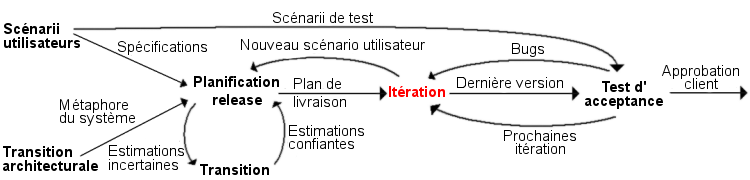
\includegraphics[width=15cm]{images/xp.png}
\caption{Cycle de l'Exreme Programing.}
\label{XP}
\end{figure}


\chapter{Rédaction des spécifications}
%- capture de fichiers
%- moulinette pour produire les KML
%- intégration dans googlearth

%Les besoins exprimé

Comme vous l'avez compris, utiliser une méthode agile comme l'extreme programming \nref{xtreme} implique une perpétuelle réécriture des spécifications. Celle ci sont améliorée, réécrite, ajoutée tout au long du projet. C'est pourquoi dans ce rapport serra cité la dernière version des spécifications.

Les spécifications du logiciel sont les suivantes:
\begin{description}
    \item[Capture de fichiers de configuration:] Les points caractéristiques, route, zone de contrôle et \textsc{Aci}, doivent être récupérés dans les fichiers de configuration du système \textsc{Tiare} afin d'avoir la représentation la plus juste de ce que le système a. Ils doivent être gardé en mémoire pendent toute l'exécution du logiciel afin de pouvoir être utilisé. Les données seront enregistrées dans des objet le temps de l'exécution du programme afin de faciliter leur exploitation. La configuration du logiciel doit laisser à l'utilisateur la possibilité de spécifier le chemin du fichier de configuration.

    \item[Capture des données Plan de vol:] Les données Plan de vol doivent être récupérées dans les log du système \textsc{Tiare}. Par contre il doit être possible de les récupérer d'un autre fichier contenant des trames \textsc{Fpl} au format normalisé par la norme 4444 (cf Bib. \cite{4444}). Chaque plan de vol serra enregistré dans un objet ayant un identifiant comprenant: L'identifiant de l'avion, son aéroport de départ ainsi que l'heure et le jour de départ. Cet identifiant a pour but de les différentier et de les référencer dans le temps. La configuration du logiciel doit laisser à l'utilisateur la possibilité de spécifier le chemin du fichier de log.

    \item[Capture des données \textsc{Ads}:] Les données \textsc{Ads} doivent être récupérées dans les log du système \textsc{Tiare}. Il devra être aussi récupérer dans ces log les points de la position en fonction du temps calculé par le système entre deux report \textsc{Ads}. Les reports \textsc{Ads} et points calculé seront instancié par avion et par vol. L'identifiant de chaque vol sera donc composé de l'identifient de l'avion ainsi que de la date et l'heure du message de login. La configuration du logiciel doit laisser à l'utilisateur la possibilité de spécifier le chemin du fichier de log.

    \item[Les points caractéristiques:] Ces points devront être implémentés dans \textsc{Google Earth} avec la possibilité de les afficher ou non. La configuration du logiciel doit laisser à l'utilisateur la possibilité de spécifier la possibilité de rééditer ou non le fichier source \textsc{Google Earth}. Ces points serons représenté par un triangle de petite taille.

    \item[Les zones de Contrôle et \textsc{Aci}:] Les zones de contrôle et zones \textsc{Aci} devront être implémenté dans \textsc{Google Earth} avec la possibilité de les afficher ou non. La configuration du logiciel doit laisser à l'utilisateur la possibilité de spécifier la possibilité de rééditer ou non le fichier source \textsc{Google Earth}. Ces zones seront représentées par une surface colorée en 2 dimension.

    \item[Les routes:] Les routes devront être implémentées dans \textsc{Google Earth} avec la possibilité de les afficher ou non. La configuration du logiciel doit laisser à l'utilisateur la possibilité de spécifier la possibilité de rééditer ou non le fichier source \textsc{Google Earth}. C'est route seront représentée par une ligne de couleur Jaune. Les points définissant cette route ne seront pas illustrés afin de ne pas faire de doublon avec les points caractéristique. Les coordonnées des points de chaque route devront être défini à partir des points caractéristique en mémoire.

    \item[Les plan de vol:] Les plans de vol devront être implémenté dans \textsc{Google Earth} avec la possibilité de les afficher ou non. La configuration du logiciel doit laisser à l'utilisateur la possibilité de spécifier la possibilité de rééditer ou non le fichier source \textsc{Google Earth}. Les plans de vol doivent pouvoir être visualisé dans \textsc{Google Earth} en fonction du temps. Pour se faire une heure théorique de passage sera calculé par le programme pour chaque point définissant le plan de vol. Toutes les informations concernant chaque plan de vol tel que ça route, les points constituant sa route et sa situation dans le temps devront être regroupé dans un dossier. Le message FPL de l'avion doit être visible dans la description de ce dossier. Les plans de vol seront visible durant toute la durée du vol et représenté par une ligne noire. La visualisation dans le temps sera représentée par un segment de couleur choisie aléatoirement pour chaque vol défini par les deux points les plus proches de l'heure en paramètre dans le logiciel (un point avant et un point après). Ce segment et ses points ne serons visible qu'à partir de l'heure du premier points jusqu'à l'heure du deuxième. 

    \item[l'intersection du plan de vol avec la zone \textsc{Aci}:] L'intersection, si elle a lieu, entre le plan de vol et la zone \textsc{Aci} doit être calculé, définie et représenté dans \textsc{Google Earth} par un point rouge accompagné du nom de l'avion et de l'heure d'intersection affiché en rouge également. Ces points devront être contenu dans le dossier du concerné.

    \item[Les report \textsc{Ads}:] Chaque report \textsc{Ads} serra composé de ces points de report ainsi que des points calculé par le système. Chaque report serra regroupé dans un dossier par vol et aura comme description le message reçu. Chaque point calculé par le système sera attribué et regroupé avec le report précèdent. Les vols seront représenté par une ligne blanche retraçant tout les report reçu, ainsi que chaque point affiché dans le temps. L'intérêt étant de visualisé l'écart entre le chemin parcouru par l'avion et le plan de vol déposé ainsi que la différence entre la trajectoire de l'avion et celle calculée par le système \textsc{Tiare}. 
\end{description}


















\chapter{Réalisation technique}
%Réalisation technique
    %Contexte technique opérationnel
        %Plan de vol et reports ADSC
        %Plate-forme TIARE (production de log fichiers texte)
    %Base de travail
        %Python : librairies, IDE, Linux
        %Google Earth
    %Conception Produit
            %Le programme réalisé et ses fonctions
                %Analyse DATASET
                %Analyse du trafic
    %Problèmes techniques rencontrés
            %Rotondité, intersection, zip, optimisation dans google earth….



Avant de passer à la pratique un apprentissage théorique à du être réalisé.

\section{Le contexte technique opérationnel}

    \subsection{\textsc{EurocatX}}
Il faut bien comprendre comment marche le système afin de bien visualiser d'où proviennent les informations. Comme décrit grossièrement dans le schéma (cf. Fig. \vref{eurocatx}),
\begin{figure}
    \center
    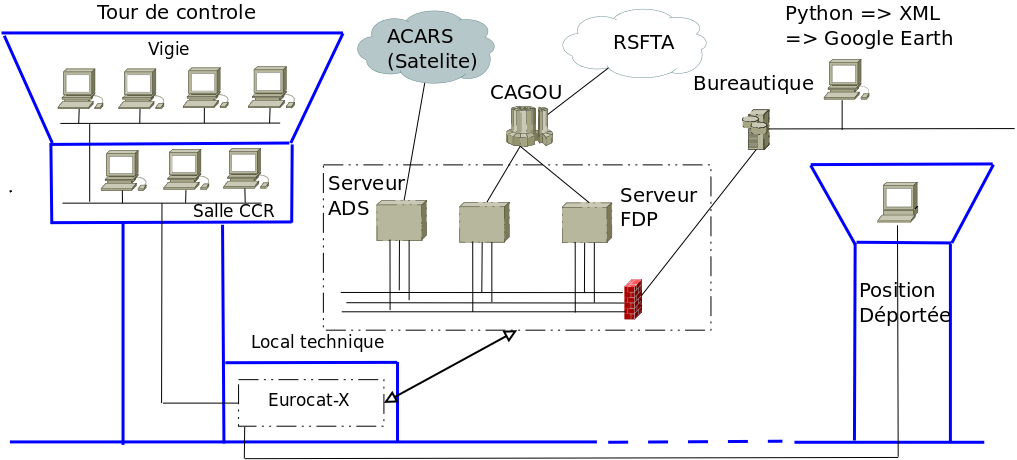
\includegraphics[width=15cm]{images/SchemaControle.png}
    \caption{Schématisation du système \textsc{EurocatX} au niveau des tour de contrôle}
    \label{eurocatx}
\end{figure}
\textsc{EurocatX} récupère les information sur les plans de vol par l'intermédiaire de \textsc{Cagou}\footnote{\textsc{Cagou}: nom donné au commutateur \textsc{Rsfta}}. Il récupère aussi le positionnement émis par l'avion à l'aide de la transmission Satellite, \textsc{Vhf}\footnote{\textsc{Vhf}: Very High Frequency, soit une bande radio de très haute fréquence} ou des données radars lors de son approche. Le système \textsc{EurocatX} donne un accès à la bureautique protégé par un par-feu (FireWall) afin de rendre disponible sur ce réseau un certain nombre d'information. Dans notre cas nous y récupérerons:
\begin{itemize}
    \item toutes les données de configuration du système tels que les nom et coordonnées des balise référencée, la position des zone de contrôle et des zone \textsc{Aci} ou encore les route utilisée pour décrire les plans de vols.
    \item Les fichiers de log du Commutateur \textsc{Cagou} afin de pouvoir exploiter les plans de vol reçus par le réseaux \textsc{Rsfta}.
    \item Tous les report \textsc{Ads} reçu par satellite et traité par le système.
\end{itemize}\medskip 
Le système envoyé les information récoltées et celle calculées au visues\footnote{Visue: Nom pour décrire les ordinateur utilisés pour visualiser les données de contrôles} situées dans la tour de contrôle au niveau de la Vigie ou de la salle \textsc{Ccr} ainsi que de la position déportée à \textsc{Morea}.

Les données seront donc récupérée dans les fichiers ".asf" pour tous ce qui est de la configuration du système, dans les fichier du \textsc{Fdp} pour les plans de vol et dans les fichiers du serveur \textsc{Ads} pour les report ainsi que pour la position calculée des aéronefs.

    \subsection{Le domaine de l'aviation}
Il m'a aussi été nécessaire de prendre connaissance de touts les terme, unité, convention et j'en passe utilisé dans le domaine aéronautique.

        \subsubsection{Les coordonnées et unités:}
Tout d'abord est vite venu le problème de conversion de coordonnées, J'ai donc du revoir les conversions de coordonnées sphériques ainsi que les conversions de distances.
J'ai également du, comme expliquée ci dessus (cf. \vref{mathcoord})
me remémoré les manière de calculé le point d'intersection de deux arc de cercle en coordonnées sphériques.

        \subsubsection{Convention:}
Plusieurs conventions on du être acquise comme celle utilisé par le système TIARE pour décrire les report \textsc{Ads} ou encre celle utilisée par les compagnie pour le dépôt de plan de vole.
NE PAS OUBLIER DE FAIRE RÉF AU DOCUMENT 4444 ...





\section{Base de travail}
    \subsection{Le langage Python}
        \subsubsection{Bien coder:\label{pygood}}
Afin de pouvoir apprendre les bonne pratique de la programmation Python j'ai lu un livre intitulé "Programmation Python, conception et Optimisation"\cite{pybook}. Celui-ci m'a permit de pouvoir d'une part revoir ce qui avait été appliquer lors de mes études et d'autre part avoir une vue global sur le langage et ainsi pouvoir prendre du recule lors du codage.

Celui ci m'a par exemple appris le nouveau style de programmation qui part du principe que chaque nouvel objet définit est basé sur un Objet existant, et que par la même occasion tout en python était Objet (même une simple variable booléenne). Ou encore la manière de vérifier si un objet était faux, égale à 0 ou encore une chaîne vide simplement en demandant si il existait (ex:~\texttt{"if x != 0:"}~devient \texttt{"if not x:"})

        \subsubsection{Utiliser les expression régulière:} 
L'apprentissage de l'utilisation des expression régulière\footnote{Une expression régulière
 est en informatique une chaîne de caractères que l’on appelle parfois un motif et qui décrit un ensemble de chaînes de caractères possibles selon une syntaxe précise.}, m'a été grandement facilité garce au site: \url{http://www.dsimb.inserm.fr/}\cite{re} et a la documentation en ligne de Python\cite{pydoc}. Il s'est avéré après apprentissage que ces expression régulière aurons grandement facilité la faisabilité du projet.

        \subsubsection{L'optimisation:}
Je pourrais cité un passage du livre\cite{pybook} qui dit:
\begin{quotation}
    Fourni dès le départ avec des modules de tests, Python est un langage agile. Le terme agile est originellement issu de la méthodologie de programmation agile (Beck et Al.), très proche de la programmation itérative. Cette méthodologie, qui réduit les risques liés à la conception de logiciels, introduit entre autres des principes de tests continus du code.
    \raggedleft Vincent \textsc{Lozano}.
\end{quotation}

En effet il m'a été rapidement nécessaire de réalisé des test, aussi bien pour vérifier que mon code était valide que pour vérifier que celui-ci s’exécutait normalement. Il c'est avéré à plusieurs reprises que certaines parties de mon code étaient très gourmandes en processus. L’apprentissage des fonction de test du code tel que le module hotshot décrit plus tard (cf. \vref{perf}) m'a été rapidement nécessaire.

    \subsection{\textsc{Google Earth}}
\textsc{Google Earth} est un logiciel, propriété de la société \textsc{Google}, permettant une visualisation de la terre en 3 dimensions avec un assemblage de photographies aériennes ou satellites. Ce logiciel donne la possibilité de configurer un environnement, ajouter des lignes, des points ou encore des polygone en 3D en passent par des fichier de configuration au format KML\footnote{\label{Kml}KML: Keyhole Markup Language, est un format de fichier et de grammaire XML pour la modélisation et le stockage de caractéristiques géographiques comme les points, les lignes, les images, les polygones et les modèles pour l'affichage dans \textsc{Google Earth}, dans \textsc{Google Maps} et dans d'autres applications.}.

Ce format, qui repose sur le XML\footnote{XML: Extensible Markup Language («langage extensible de balisage»), est un langage informatique de balisage générique.}, a l'avantage d’être simple à manipuler. Ça sémantique est définie sur le de google (cf. Bibliographie \cite{gecode}) 



\section{Le programme réalisé et ses fonctions}
    \subsection{Le fonctionnement}
            \paragraph{La configuration:}
Le programme réalisé ne possède pas encore d'interface (IHM) graphique. Il est donc nécessaire de configurer les option a l'aide d'un fichier de configuration (cf. annexe \vref{config}). Nous pourrons régler par l'intermédiaire de celui-ci:
\begin{itemize}
    \item Les fichiers Kml à recréer ou non, se qui est utile afin de ne pas avoir à recréer des fichier statique (tel que la position des point caractéristique ou encore des zones de contrôles) a chaque utilisation tout en laissant a l'utilisateur la possibilité de les mettre a jour simplement.
    \item Les différant styles et couleurs.
    \item L'emplacement des fichiers de configuration.
    \item les description et noms appliqué à chaque catégorie.
\end{itemize}\medskip
            \paragraph{L'exécution:}
Le fichier de configuration renseigné, le programme peut être lancé. Il est possible de le lancer par l'intermédiaire d'un Shell\footnote{Shell: Interface en lignes de commandes}, par l'intermédiaire de l'interface Python ou encore en direct si les information pour gérer et lancer les fichiers Python ont été renseignée dans le système d'exploitation.
            \paragraph{Le résultat}
L'exécution du programme réalise une suite d'action:
\begin{enumerate}
    \item Lire le fichier de configuration afin de déterminer les action a effectuer.
    \item Lire les fichiers de configuration du système \textsc{Tiare} affin de récupérer toutes les variable nécessaire sous forme d'objet\footnote{Objet: structure de données valuées et cachées qui répond à un ensemble de messages. Cette structure de données définit son état tandis que l'ensemble des messages qu'il comprend décrit son comportement} (ex: points caractéristique ...)
    \item Lire les fichiers de log afin de créer des objets tel que les plans de vol ou encore les report \textsc{Ads}. Ces objet sont créer non seulement a partir de ses fichiers de log mais aussi a partir des objets créer précédemment (ex: les point des plan de vol désigné par un nom sont convertis en coordonnées à l'aide des points caractéristiques).
    \item Créer les fichier \textsc{Kml} désigné dans le fichier de configuration à l'aide des objets instancié.
    \item Créer un fichier \textsc{Kmz} a l'aide de tout les fichiers \textsc{Kml} afin d'avoir un fichier compact et facile a transporter.
\end{enumerate}


\section{Problèmes techniques rencontrés et solution apportées}
Comme dans tout projet il y a une une multitude de problèmes a résoudre. Nous verrons dans cette partie quelques exemples de ces problèmes rencontré ainsi que la manière dont il ont été résolus. Cette liste reste bien entendu exhaustive au regard de tout les petit problème auxquels nous avons du faire face.

    \subsection{Gestion des erreur}
            \paragraph{problématique:}
Le premier problème que nous avons rencontrer a été celui de la gestion des erreur. En effet, de la première mise en route du logiciel jusqu'à la fin du stage des erreurs ont du êtres gérée. Deux type d'erreur sont revenue:
\begin{itemize}
    \item Le premier type d'erreur était par exemple une réaction in attendue du logiciel, On pourrait prendre en exemple la conversion de coordonnées reçue en Système sexagésimal \footnote{(Système sexagésimal : Degrés ( \degres\ ) Minutes ( ' ) Secondes ('' ))} en coordonnées utilisées dans les fichiers KML \vref{Kml}, qui lors des premiers test donnais des donnée erronées.
    \item Le deuxième type était celui du au erreur contenu dans les fichiers de log utilisé pour récupérer les informations. Ces erreur faisait effet boule de neige et venait se répercuter dans le fonctionnement du logiciel.
\end{itemize}\medskip

            \paragraph{Résolution:}
La solution au premier problème a été de mettre en place des test a chaque fonction implémenter ou après avoir réaliser chaque objectif fixé. On appel cette méthode le test continu du code. Grâce à cela nous allons pouvoir déterminer plus rapidement lors d'une erreur futur d'où provient celle-ci. Une méthode simple de la mette en place est de définir un test a réaliser pour valider la fonction ou le code. On détermine donc quel réaction doit avoir un fonction pour un environnement donné et l'on vérifie si le résultat corresponds bien avec celui espéré. (Ex: on a la coordonnée 4530N10045E qui correspond a 45\degres 30' Nord 100\degres 45' Est. On envoi cette variable dans la fonction de conversion et l'on vérifie que le résultat retourné est bien en décimal: 45,5\degres\ en latitude et -100,75 en longitude). Si le résultat est correct la fonction ou le morceau de code est validé, sinon il doit être corrigé.
La solution du deuxième problème a été dans un premier temps d'afficher chaque erreur dans la console, mais cela est vite devenu trop compliqué du fait que la console ne retient par défaut qu'un nombre limité de ligne en mémoire et que les ligne trop ancienne sont simplement effacée. On a donc mis en place un système de log permettant, en plus d'avoir accès au information les plus ancienne, de pouvoir l'exploiter ares avoir fermé la console, effectuer des recherche a l'intérieur et tout avantage que peut apporter un fichier texte. Pour les dernière version de log, celles-ci sont crées avec des information relative au type d'erreur et l'emplacement de l'erreur dans le fichier source, le tout enregistrées dans un fichier comprenant la date et l'heure actuel dans le nom afin de pouvoir les différencier de chaque exécution du logiciel. 

    \subsection{Intersection entre plans de vol et zone ACI\label{mathcoord}}
            \paragraph{Problématique:}
Afin de déterminer l'heure d'entrée approximative des avions dans la zone ACI (cf. \vref{Aci}) en fonction de leur plan de vol déposé Il est nécessaire de déterminer le point d'intersection entre leur plan de vol et la zone ACI. En théorie cela paraît simple, il suffit de prendre chaque portion du trajet du plan de vol composé de deux point et formant une droite, et  de déterminer si cette droite coupe chaque droite composant la zone ACI. Dans la pratique il c'est avéré que cela était un peu plus compliqué, en effet ces droites sont en réalité des arcs de cercles qui sont composé de deux extrémités définies par des points en coordonnées sphériques (cf. schéma fig. \vref{sphere}).
\begin{figure}
    \center
    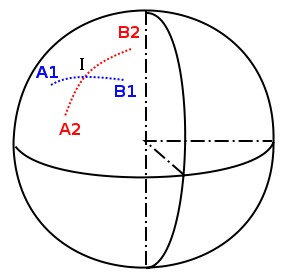
\includegraphics[width=5cm]{images/Sphere.png}
    \caption{Représentation grossière de l'intersection de deux arc de cercle respectivement formé par la trajectoire la plus courte entre deux points situé sur le Globe terrestre}
    \label{sphere}
\end{figure}
            \paragraph{Résolution:}
Étant donné que j'ai effectué un BTS avant d'intégrer l'EIGSI \footnote{EIGSI: École d'Ingénieurs en Génie des Systèmes Industriel située à La Rochelle}, les notion de coordonnées sphérique ne me sont que peut familière. Après avoir en vainc cherché sur internet ainsi que dans mon entourage  (maître de stage, collègues de travail) je me suis replié sur un forum de mathématique sur le quel j'ai déposé un sujet explicitant le problème (adresse, cf. bibliographie \cite{forummath}). Une personne nous a donnée une solution qui, après connaissance, semble tellement simple qu'on se demande pourquoi personne n'y a pensés. Cette solution consiste a déterminer les plan défini par les deux points aux extrémités de chaque arc et par le centre de la terre (ainsi nous avons forcement la courbe qu'a suivi l'avion sur ce plan). Il faut ensuite déterminer la normal a chacun des plan pour en déduire la droite d'intersection de ces plan (passant par le centre de la sphère). Une foi cette droite acquise il faut définir sont vecteur norme et le convertir en coordonnée sphérique. Ce qui nous donne un des point d'intersection de la droite avec la sphère, l'autre étant situé par définition à l'opposé.

Une démonstration valant amplement un long discours, et a titre informatif, voici ce que cela donne en résolution mathématique. Pour cet exemple nous avons deux arcs représentent 2 trajectoires définies chacune par 2 points A et B (cf. Fig. \vref{sphere}). Chaque pour sera défini par une latitude et une longitude.

Nous avons donc:
\begin{itemize}
    \item $lat_{A}$ la latitude de A
    \item $long_{A}$ la longitude de A
    \item $(x_{A}, y_{A}, z_{A})$ les coordonnées cartésiennes de A
    \item $I_{1}$ le point d'intersection \no 1
    \item $I_{2}$ le point d'intersection \no 2
\end{itemize}
Il faut tout d'abord convertir les coordonnées sphérique en vecteur de coordonnées cartésiennes pour $A$ et $B$:
$$  A=\left\{
\begin{array}{rcl}x_A & = & cos(lat) \times cos(long)\\ y_D & = & cos(lat_{A}) \times sin(long_{A})\\ z_A & = & sin(lat_{A}) 
\end{array}\right.$$
Il faut ensuite déterminer le plan passant par $O$, $A$ et $B$ ayant alors pour équation:
$$ax+by+cz=0$$ où $$\left(\matrix {a\cr b\cr c}\right)= \left(\matrix {x_A\cr y_A\cr z_A}\right)\wedge \left(\matrix {x_B\cr y_B\cr z_B}\right)$$c'est à dire $$\left\{\matrix {a=y_Az_B-z_Ay_B\cr b=z_Ax_B-x_Az_B\cr c=x_Ay_B-y_Ax_B}\right.$$
L'intersection des deux plans de coordonnées $(a,b,c)$ et (a',b',c') contient le point O, mais aussi le point $P$ de coordonnées $(x_P,y_P,z_P)$ tel que: $$\left(\matrix {x_P\cr y_P\cr z_P}\right)= \left(\matrix {a\cr b\cr c}\right)\wedge \left(\matrix {a'\cr b'\cr c'}\right)$$
P n'étant pas forcément sur la sphère, il faut trouver un point de la droite $(OP)$ sur cette sphère. Pour cela il suffit de diviser les 3 coordonnées de P par la norme de $\overrightarrow{OP}$:
$$I_{1} = \left\{\matrix {x_P / \sqrt{x_P^2+y_P^2+z_P^2}\cr x_P / \sqrt{y_P^2+y_P^2+z_P^2}\cr x_P / \sqrt{z_P^2+y_P^2+z_P^2}}\right.$$
nous avons donc $I_1$ et son opposé $I_2$, il nous reste donc plus qu'a vérifier si chacun de ces points appartient à un des 2 arcs.

Vous trouverez le code Python correspondant à ces calcule dans la fonction: "verifyIntersection (line, point):" du module "ususalFonction.py" disponible en annexe \vref{usualfonction}

    \subsection{Performance du logiciel\label{perf}}
            \paragraph{Problématique:}
Les premiers tests du logiciel ce sont déroulé sur un nombre limité de fichiers (représenté par un nombre limité d'heure de vol), ce affin de pouvoir les valider rapidement. Lors de l'apparition de fichiers plus volumineux (plus de 300Mo de donnée en entrée, environ 10\% en sortie) c'est posé le problème de performance. Avant optimisation l'ordinateur moulinais des heures avant de pouvoir sortir un fichier. Il a donc fallût optimiser le code afin d'alléger le programme en ressources.

            \paragraph{Résolution:}
En cherchant des conseils dans des forum d'informatique ainsi que dans le livre cité précédemment (cf. bibliographie \cite{pybook}, nous avons découvert que Python était un langage orienter par les test et qu'il disposait donc de librairies spécialement conçues pour déterminer les point bloquant d'un programme et les fonctions appelées les plus gourmandes.

La fonction retenue pour repérer ce qui est appelé en anglais les Bottleneck\footnote{Bottlneck: (goulot d'étranglement) point d'un système limitant les performances globales, et pouvant avoir un effet sur les temps de traitement et de réponse.} est la fonction "hotshot" qui à pour but d'analyser un programme dans sa totalité en indiquant notamment les ressources utilisées par chaque fonction appelée. Pour visualiser ce que donne le résultat d'une analyse veuillez vous reporter a la figure \vref{stat}.

Les bottlenecks repérés, une réécriture des parties bloquantes à du être effectuée. Cette analyse nous a permis de réduire les ressources et donc le temps d'exécution du logiciel de plus de 80\%.


\chapter{Tests et validation de la réalisation}
%Tests et validation de la réalisation
%            Démarche pour tester le produit (manque pas des vols)
%            Un fichier même vol, mais fichiers avec des vols supplémentaires
%            Présentation du rendu
%Améliorations continues : à partir des tests, je repars dans le chapitre précédent (réalisation technique + nouveaux besoins (comparaison FPL//ADSC) ou correction)

\section{Les tests}
Nous avons effectué au cours de ce projet deux types de tests: les tests unitaires et les tests globaux.

    \subsection{Les tests unitaires}
En programmation informatique, le test unitaire est un procédé permettant de s'assurer du fonctionnement correct d'une partie déterminée d'un logiciel ou d'une portion d'un programme (appelée «unité» ou «module»).

On écrit un test pour confronter une réalisation à sa spécification. Le test définit un critère d’arrêt (état ou sorties à l’issue de l’exécution) et permet de statuer sur le succès ou sur l’échec d’une vérification. Grâce à la spécification, on est en mesure de faire correspondre un état d’entrée donné à un résultat ou à une sortie. Le test permet de vérifier que la relation d’entrée - sortie donnée par la spécification est bel et bien réalisée.

Rappel de définitions :
\begin{description}
\item[Test:] il s'agit d'une vérification par exécution.
\item[Vérification:] ce terme est utilisé dans le sens de contrôle d'une partie du logiciel. (Une «unité» peut ici être vue comme «le plus petit élément de spécification à vérifier»)
\end{description}

Il s'agit pour nous de tester un module, indépendamment du reste du programme, ceci afin de s'assurer qu'il répond aux spécifications fonctionnelles et qu'il fonctionne correctement en toutes circonstances.

Mais ces tests ne sufisent pas car il ne donnent pas assez de recule pour visualiser si l'ensemble du programme est fonctionnel. Il nous donne seulement une confirmation théorique.

    \subsection{Les tests globaux}
Comme nous l'avons cité précédement des tests unitaires ne sont pas sufisant dans notre cas. En effet ce projet étant un réél prototype, dans le sens ou rien n'a été effectué de semblable auparavant, les spécifications restent parfois mal déterminées. On pourra citer comme exemple la structure des messages \textsc{Fpl} qui sont cencés avoir toujours la même forme, mais qui se retrouve souvent avec des erreurs dûes à la qualité de transmission.

Ces tests auront donc pour but de valider le fait que toutes les parties développées indépendamment fonctionnent bien ensemble de façon cohérente.

Pour ce faire nous avons passé un grand nombre de fichiers sources à «parsé». Ce qui nous a permis de découvrir tout au long du projet un certain nombre d'erreurs. Nous pourons citer en exemple le fait de prendre en compte le nom de l'avion, aéroport de départ et heure de départ comme identifiant, celui-ci pouvant être le même sur plusieurs jours pour les vols cylciques. Dans ce cas les tests globaux nous ont permis de découvrir l'errure et nous ont permis d'ajouter le jour de départ de l'avion dans l'identifiant afin que chaque identifiant reste bien unique.

\section{La validation}
Chaque fin de cycle de notre méthode de gestion de projet qui est l'Extreme Programing nous amène à une étape de validation. Celle-ci conciste à verifier avec le client que le programme se comporte bien comme il le souhaitait.

Après chaque validation des spécifications sont modifiées car, bien que répondant à leur definition, elles ne répondent pas réelement aux attentes du client. D'autres spécifications sont crées et certaines annulées.

\section{Amélioration continue}
A partir des tests réalisés et de la validation avec le client comme cité précédement nous redéfinissons les besoins ainsi que les spécifications. Cela nous amène donc à revenir au cycle des besoins \nref{besoins} dans notre méthode de gestion de projet \nref{extreme}.

Nous reprenons alors un cycle ce qui nous permettra d'améliorer le programme en continu.




\chapter{Synthèse}
Synthèse
Méthode employée à consommateur de personne à disposition, produit très riche si compétence,  adapté et performant, Evolution désordonnée si pas maitrisé (base de données en plus ), changement des spécifications  en cours de projet, difficulté de rédaction de spécification produit fini concentre sur le dev et moins sur la doc.
Pas de rédaction de manuel d’utilisateur,


\chapter{Evolution projet}
\label{evolution}
Ce projet est loin d'être arrivé à terme. Nous allons donc voir ici ce qui pourrait être fait afin de perfectionner ce logiciel. Les évolutions seront axées sur trois points:
\begin{itemize}
    \item La mise en place d'une interface graphique.
    \item L'automatisation de l'acquisition.
    \item La pérennisation des données.
\end{itemize}

\section{La mise en place d'une interface graphique}
Comme il a été expliqué précédemment \nref{fonctionnement}, la configuration du logiciel est effectuée manuellement par l'intermédiaire de fichiers textes et son exécution est effectuée en ligne de commande. C'est pourquoi une interface graphique faciliterait grandement son utilisation.

Cette interface devrait pouvoir faciliter la configuration et l'exécution du programme, elle pourrait être basée sur des technologie web afin de la rendre portable tout en séparant le traitement des données de l'utilisation du fichier final dans \textsc{Google Earth}. En effet le programme pourrait être lancé a distance sur une machine, cela permettrait de sécuriser l'accès au données tout en libérant les ressources du poste de l'utilisateur.

Pour faciliter la configuration un histogramme avec tous les vols figurant entre deux dates sélectionnées pourrait être réalisé, cela permettrait de mieux visualiser le trafic et de pouvoir cibler les vols à afficher.

Il pourrait aussi être intéressant d'inclure l'affichage final dans l'interface web, tout en laissant la possibilité à l'utilisateur de télécharger le fichier afin d'exploiter pleinement toutes les fonctionnalités du logiciel \textsc{Google Earth} tel que la mesure de distance entre deux points.

\section{L'automatisation de l'acquisition}
Actuellement chaque fichier à traiter est récupéré manuellement. On pourrait concevoir un système qui irait de lui même chercher les fichiers nécessaires dans le système \textsc{Tiare} et les mettre automatiquement à la disposition du programme.

\section{La pérennisation des données}
Dans une optique de pouvoir rejouer simplement des situations passées, on pourrait mettre en place un système de base de données légère tel que SQLite\footnote{SQLite est une bibliothèque écrite en C qui propose un moteur de base de données relationnelles accessible par le langage SQL.}. Contrairement aux serveurs de bases de données traditionnels, comme MySQL ou PostgreSQL, sa particularité est de ne pas reproduire le schéma habituel client-serveur mais d'être directement intégré aux programmes. L'intégralité de la base de données (déclarations, tables, index et données) est stockée dans un fichier indépendant de la plate-forme.

Ce procédé couplé à un traitement automatique permettrait de mettre et garder en mémoire tous les vols disponibles sur le système \textsc{Tiare}. Il permettrait donc de pouvoir rejouer des situations qui ont été enregistrées plusieurs mois avant. 





% Bibliographie
\bibliographystyle{plain}
\bibliography{tex/biblio}

% Début annexes
\appendix
%%Prévoir une annexe avec la description de l’ADSC / CPDLC

\section{Les codes sources du projet}
    \subsection{Main}
Ce fichier sert à executer tout le programme:
\lstinputlisting{/home/manu/DTI/Manu.py}
    \subsection{Config}
Nous avons ic le fichier de configuration. Celui ci sert notament à se passer temporairement d'une interface graphique.
\lstinputlisting{/home/manu/DTI/manu.cfg}
    \subsection{KML}
Afin de pouvoir réaliser les document KML, un module a été implémenté. Celui-ci a pour objectif de mettre en forme le document final. Il ne réalise aucun calcul. Lors de l'initiation une variable est instencié. Celle-ci accumulera toute la mise en forme du document jusqu'a l'appel de la foction de fin qui permettera de clore cette variable et de l'enregistrer dans un fichier texte.
\lstinputlisting{/home/manu/DTI/modules/KML.py}

%\section{Anexes}
%%¯¯¯¯¯¯¯¯¯¯¯¯¯¯¯¯¯¯¯¯¯¯

%\input{lynx}
%\input{disquettes}

\end{document}



